\def\year{2015}
%File: formatting-instruction.tex
\documentclass[letterpaper]{article}
\usepackage{aaai}
\usepackage{times}
\usepackage{helvet}
\usepackage{courier}
%%
\usepackage{graphicx}
\usepackage{url}
\usepackage{amsfonts}
\usepackage{moreverb}
%%
\usepackage{bm}
\usepackage{paralist}
%%
% so we don't need to specify figures subdirectory in figure code
\graphicspath{{./figures/}}
\usepackage{subfig}

%needed to change table colors
\usepackage[table]{xcolor}
%%
\frenchspacing
\setlength{\pdfpagewidth}{8.5in}
\setlength{\pdfpageheight}{11in}
\pdfinfo{
/Title (Insert Your Title Here)
/Author (Put All Your Authors Here, Separated by Commas)}
\setcounter{secnumdepth}{0}  
 \begin{document}
% The file aaai.sty is the style file for AAAI Press 
% proceedings, working notes, and technical reports.
%
\sloppy{
\title{Spoken Dialog Systems for Health Interventions using Fully Autonomous Humanoid Robots}
%\author{Saminda Abeyruwan\\
%University of Miami\\
%Dept. of Computer Science\\
%Coral Gables, FL 33146\\ 
%saminda@cs.miami.edu\\
%\And  Ramesh Baral\\
%Florida Int'l University\\
%Comp. \& Info Science\\
%Miami, FL 33199 \\
%rbara012@cis.fiu.edu\\
%\And Ugan Yasavur\\
%Florida Int'l University\\
%Comp. \& Info Science\\
%Miami, FL 33199 \\
%uyasa001@cis.fiu.edu\\
%\And Christine Lisetti\\
%Florida Int'l University\\
%Comp. \& Info Science\\
%Miami, FL 33199 \\
%lisetti@cis.fiu.edu\\ 
%\And Ubbo Visser\\
%University of Miami\\
%Dept. of Computer Science\\
%Coral Gables, FL 33146\\
%visser@cs.miami.edu\\
}



\maketitle
\begin{abstract}
We combined a spoken dialog system that we developed to deliver brief health interventions with a 
3D anthropomorphic speech-enabled interface to a fully autonomous humanoid robot (NAO). The dialog 
system is based on Markov decision processes (MDPs). We use off-policy algorithms in 
reinforcement learning (RL) with the data  collected from real user interactions to obtain the 
(near-) optimal policy. The system begins to learn optimal dialog strategies for initiative 
selection and for the type of confirmations that it uses during the
interaction. The health intervention framework, delivered by a 3D character instead of the 
NAO, has already been evaluated, with statistically significant results in terms of task 
completion, ease of use, and future intention to use the system.  The current spoken dialog system 
for the humanoid robot is a novelty and exists so far as a proof of concept.
\end{abstract}

%Keywords Spoken dialog Systems á Reinforcement Learning á Virtual Agents and Avatars á Behavior
%Change Brief Intervention

\section{Introduction} \label{intro}

%Spoken dialog systems (SDS) and autonomous humanoid robots are emerging fields of research which, {\em together}, could bring a revolution to human-robot interaction as we know it. 
Latest developments spoken dialog systems (SDS) show complementary progress for the development of  embodied conversational agents (ECA) \cite{YASCLL14}. Yet, very little of
this progress has been used for autonomous humanoid robots, which have also recently demonstrated the ability
to serve in health interventions. The
humanoid robot NAO specifically has been used in a variety of applications in the health domain (e.g.,
\cite{MAJA13}) including user studies which demonstrate the usefulness of the NAO platform.

Dahl and Boulos (2013) \nocite{robotics3010001} gave a recent overview of how robots are used in
healthcare. Apart from the  surgical robots that are tele-operated by a human doctor, robots support
the daily work in hospitals, mainly in logistics (e.g., Atheon TUG platform \cite{bloss2011mobile}
or HelpMate \cite{evans1998helpmate}). Several other studies have looked at different autism
spectrum disorders. The main goal is to provide therapy with the help of an intelligent robotic
agent that improves both social and communication skills of the children involved. One example is
the KASPAR robot \cite{robins2012scenarios}. Its creators use robot-based play scenarios that can
be tailored for types of disability and skill areas that need to be motivated. Another example has
been created by Bekele and colleagues. They focus on communication behaviors, in particular
head-tracking to manifest the robots engagement in the on-going interaction \cite{bekele2013step}.  

There are also several studies involving the humanoid robot NAO. Csala and colleagues, for example,
studied the effectiveness of a tele-operated NAO humanoid robot in improving the wellbeing of
children having undergone marrow-transplants. Although there is no conversation with the user
involved, the study demonstrated that the NAO robot is well suited for this task due to its small
size and robustness \cite{Csala2012}. Also, the study identified personalization as a key
requirement for success. The NAO robot has also been used by Belpaeme and colleagues who used the
robot to both entertain and educate children suffering from diabetes in a hospital environment
\cite{belpaeme2012multimodal}. This work is interesting to our approach as it is focused on
providing high levels of robot autonomy using a natural language interface and a long-term memory
structure that allowed children to develop a personal relationship with the robot. Both studies by
Csala and colleagues and Belpaeme and colleague took place in hospitals, and both efforts were
greatly appreciated by the children involved.

Research in SDS has shown in the past few years that using Reinforcement Learning (RL) with MDPs for dialog management outperforms older hand-crafted rule-based approaches \cite{frampton2009,young2013pomdp}. Intelligent robotics agent researchers have not yet integrated these results in their dialog systems to our knowledge. Most systems usually involve spoken dialog, and their dialog management usually still relies on hand-crafted methods \cite{morbiniFlores2012,Bickmore2010}. 

% {\color{red}
% \textbf{FixMe}
% \begin{enumerate}
%  \item I think we would need to get references on robot dialog systems in our next version 
% if we're accepted.
%  \item We also need to have a reminder description of why is it important to run the dialog system 
% on the robot.  
% \end{enumerate}
% }

In this paper, we discuss a new mode of delivery - a spoken dialog system coupled with a NAO robot - for health interventions that can help people adopt healthy lifestyles.  The dialog system can deliver brief health interventions (BI), which are short, well structured, one-on-one counseling sessions, focused on specific aspects of problematic lifestyle behavior (e.g. overeating, poor diet, heavy drinking). BIs, which are top ranked out of 87 treatment styles in terms of efficiency \cite{miller2002mesa} and which can be delivered in 3-5 minutes \cite{Moyer2002}, assess a person's problem behavior, and provide advice about ways to eliminate it. 


\section*{Approach}

In this section we briefly discuss about the approach that have used to develop the dialog 
agent (for more detail discussion, the user is referred to \cite{YASCLL14}) . According to the 
clinician's guide for conducting brief interventions from the National Institute on Alcohol Abuse 
and Alcoholism (NIAAA) \cite{national2007helping}, a brief intervention for alcohol-related health 
problems can be delivered in three sequential steps (Figure 
\ref{fig:dialog_manager}): \begin{inparaenum}[1)] \item {\em Screening} about alcohol use; \item 
{\em Assessing} for alcohol use disorders in two sequential processes; \begin{inparaenum}[a)] \item 
assessment about alcohol {\em abuse}; and \item assessment about alcohol {\em 
dependence}\end{inparaenum}; \item {\em Advising} and assisting the state of the user according to 
the degree of alcohol problem which leads to; \begin{inparaenum} \item advice for {\em at-risk} 
drinkers; \item and advice for drinkers with alcohol use {\em disorder}. \end{inparaenum} 
\end{inparaenum}

The development of the brief intervention content is based on the guide provided by 
NIAAA \cite{national2006niaaa}. The goal of the dialog agent is to deliver alcohol screening and 
brief interventions based on this guide. Each stage contains a set of questions. The screening stage 
uses 5 questions to access state of the user with respect to alcohol consumption.  If the user 
expresses that (s)he is not consuming alcohol from time to time, the interaction is gracefully ended 
by with advice, otherwise, the the dialog continues to the assessing state.  

The assessing stage consists of two sequential processes: \begin{inparaenum}[1)] \item the 
assessment of abuse process, where, there are 4 questions to assess alcohol abuse indicators.  It is 
enough to find one indicator of alcohol abuse (e.g., risk of bodily harm, relationship trouble) to 
move to \item the assessment of dependence process (e.g., keep drinking despite problems, not able 
to stick to drinking limits). If the system can not find any indicator of abuse with the 4 
questions, it passes to the dependence process, which has  7 questions to access the users state. 
\end{inparaenum}

It is enough to detect 3 dependence indicators to transit to advice stage 
for drinkers with alcohol use disorder.  If the system does not detects 3 dependence 
indicators, it transits to advice for at-risk drinkers. Therefore, the dialog branches to two 
separate steps at the end of the assessing stage. In both branches, the system provides information 
related to the assessment of the system.  If the system assessed that the user has an alcohol use 
disorder, it refers the user to treatments such as asking  the user if she or he is ready to 
change, and suggests a goal toward a change of drinking patters, based on the user's readiness. If 
the user is an at-risk drinker, it gauges his or her readiness to change, and provides feedback and 
information about the person's drinking. Therefore in both stages, the system provides factual 
information about the person's drinking and suggested drinking limits, and asks what is the user's 
intention to change with a single question.  In total there can be a maximum of 18 different 
questions in a complete session.   

\begin{figure}[!t] 
\centering 
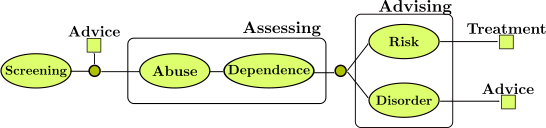
\includegraphics[width=.45\textwidth]{figures/dialog_manager} 
\caption{Dialog structure for brief interventions.} 
\label{fig:dialog_manager} 
\end{figure}

{ \color{red}
\textbf{FixMe:}
\begin{enumerate}
 \item A description of the RL method. 
 \item One simulated dialog example from the robot or 3D character. I prefer from the robot. 
\end{enumerate}
}


\section*{Implementation} 

Our implementation is based on two system designs that have been
invented and developed in two different research groups and independently. The FIU Affective Social Computing group has developed a dialog manager that is integrated in a system using a virtual 
character.  Our system utilizes the users natural speech as one input parameter and also uses gaze
and non-verbal cues for the classification of the users state. The dialog manager operates with five
interconnected MDPs representing each step or phase of the behavior intervention 
\cite{YASCLL14}. The dialog manager uses domain specific dialog phrases, a tailored grammar for
this case and a RL engine that learns over time how to address/answer to the user. It has been
successfully tested with 87 users for the alcohol domain.

The University of Miami's autonomous robots research group develops methods for both simulated and
physical agents that act in dynamic, adversarial, and real-time environments. The group uses the
RoboCup domain as an area of investigation. One  focus is on appropriate consideration of agent's
actions/behavior in order to make own decisions (for the own team agents). The group has developed a
fully implemented system (RoboCanes software) using six NAO robots that not only move in the
mentioned environment on their own, but also have to consider team communication (e.g. for global
object positions such as the ball or an opponent agent) and cooperation. The software is stable and
robust and is used as part of the backbone for this research paper.

We ported the dialog manager on one of our NAO robots. The software runs as a single process. The
dialog manager is connected to another process on the robot that makes use of CMU's Sphinx speech
recognizer system. We use the pocketsphinx 0.8 system, which is a flexible hidden Markov model-based
speech recognition system \cite{huggins2006pocketsphinx}. We also use the Sphinx 5.0 english (US)
standard language model without training or domain specific grammars.  The original dialog system described in \cite{YASCLL14} has a language model and grammars, which we plan to  adapt for the NAO robot in our next system version. A third process is the
RoboCanes software that can be connected to the dialog. Figure \ref{fig:system} gives an overview of
the architecture and the three processes. Process 1 runs as a server that is connected to process 2
via a TCP/IP connection. The robot receives a greeting mechanism  at the beginning of a conversation
that can be altered when starting again. The NAO robot then uses NAOqi for the Text-To-Speech
generation, although we have also implemented and tested other systems such as Festival \cite{taylor1998architecture} or eSpeak \cite{eSpeak},
which would also work. Process 2 then makes use of the RoboCanes framework (the RoboCup agent) which
is responsible for robot motions and also for the image processing and the audio feedback (no 
feedback from cameras at the moment yet). The robot then uses pocketsphinx, turns the audio signal
into text and sends it back to the dialog manager. The timing between processes 1 and 2 are based on 
turns, process 3 runs with 100 Hz for the joint requests and 30 Hz for both cameras.

\begin{figure}[!t] 
\centering 
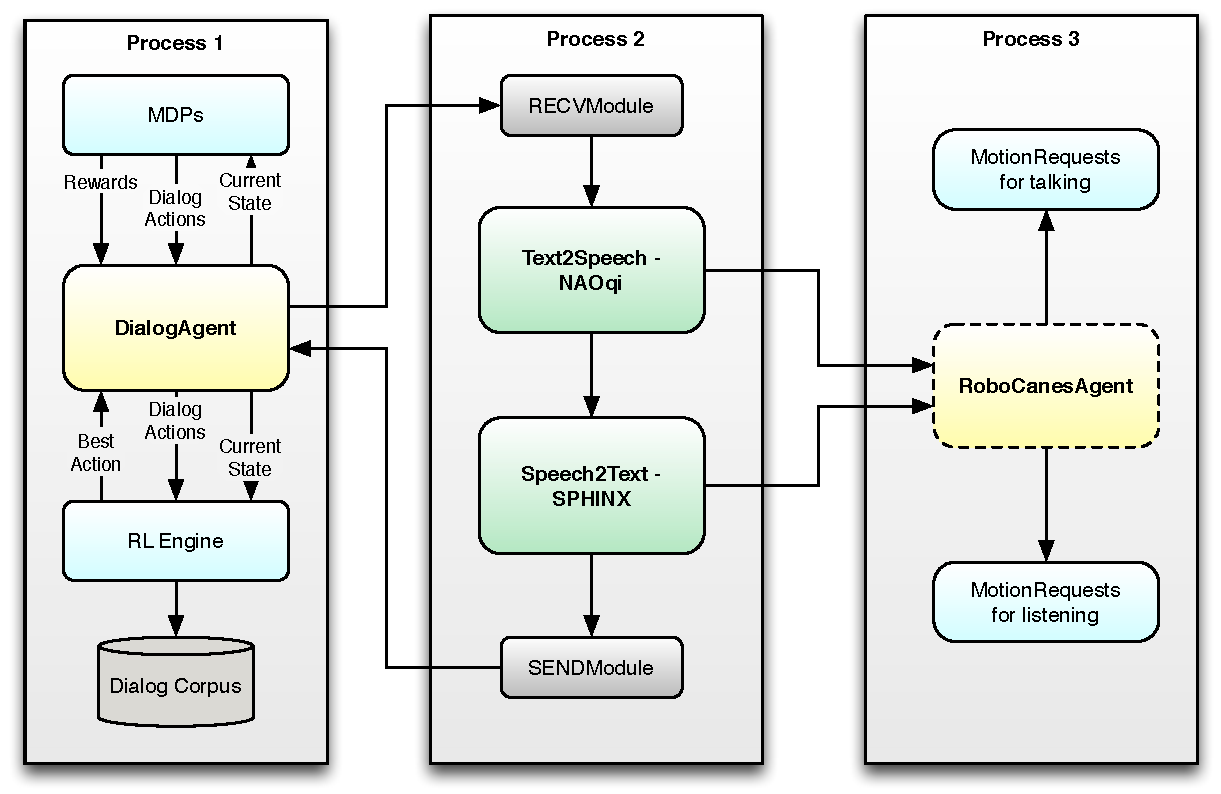
\includegraphics[width=.45\textwidth]{figures/system} 
\caption{System Architecture: process 1 contains the dialog manager, process 2 delivers speech from 
the robot and
the recognition of the human, whereas process 3 is responsible for motions that accompany the 
robot's
speech and listening time.} 
\label{fig:system} 
\end{figure}


\section*{Conclusions} 

Although currently at the prototype stage, we anticipate that the NAO robot will become a very 
likable and effective mode of delivery for brief interventions for target behaviors such as poor 
diet, overeating, or lack of exercise, among others.  The appeal of the NAO to children 
\cite{belpaeme2012multimodal} makes it particularly suitable to become a child's favorite health 
coach, say, to discuss eating more fruits and vegetables on a daily basis. Our platform 
provides the additional advantages such as a dialog system for a lack of exercise or  it can 
also demonstrate physical exercises.


\section*{Acknowledgement}
{\color{red}
FixMe:
}

\bibliographystyle{aaai}       
\bibliography{library}   


\end{document}
